\documentclass[makeidx, 10pt, oneside, onecolumn, openright, final, svgnames, dvipsnames, extrafontsizes]{memoir}
\usepackage[legalpaper, portrait, margin=0.1in]{geometry}

\usepackage[
   HomeHTMLFilename=index,     % Filename of the homepage.
%   HTMLFilename={node-},       % Filename prefix of other pages.
%   IndexLanguage=english,      % Language for xindy index, glossary.
%   latexmk,                    % Use latexmk to compile.
%   OSWindows,                  % Force Windows. (Usually automatic.)
   mathjax,                    % Use MathJax to display math.
]{lwarp}

\usepackage{xcolor, amssymb}
\usepackage{hologo, mflogo, calligra, dashrule}
\usepackage{tikz, comment}
\usepackage{varwidth} % hyphenate texts in TikZ Node (back cover)
\usetikzlibrary{fadings, shadings, shadows, decorations, decorations.footprints, calc, positioning, mindmap,arrows, patterns, arrows.meta}
\usepackage{fontspec}
\usepackage[misc]{ifsym}
\usepackage{multido}
\usepackage[colorlinks=true, linkcolor=BurntOrange, linktoc=all]{hyperref}
\usepackage{tfrupee}

\usetikzlibrary{
  arrows,
  calc,
  fit,
  patterns,
  plotmarks,
  shapes.geometric,
  shapes.misc,
  shapes.symbols,
  shapes.arrows,
  shapes.callouts,
  shapes.multipart,
  shapes.gates.logic.US,
  shapes.gates.logic.IEC,
  circuits.logic.US,
  circuits.logic.IEC,
  circuits.logic.CDH,
  circuits.ee.IEC,
  datavisualization,
  datavisualization.formats.functions,
  er,
  automata,
  backgrounds,
  chains,
  topaths,
  trees,
  petri,
  mindmap,
  matrix,
  calendar,
  folding,
  fadings,
  shadings,
  spy,
  through,
  turtle,
  positioning,
  scopes,
  decorations.fractals,
  decorations.shapes,
  decorations.text,
  decorations.pathmorphing,
  decorations.pathreplacing,
  decorations.footprints,
  decorations.markings,
  shadows,
  shadows.blur,
  lindenmayersystems,
  intersections,
  fixedpointarithmetic,
  fpu,
  svg.path,
  external,
}



\newcommand*{\RaisedText}[1]{%
  \begingroup
    \leavevmode
    \rlap{\kern-1pt\raise.5pt\hbox{\color{white}#1}}%
    \rlap{\kern1pt\raise-.5pt\hbox{\color{black}#1}}%
    \hbox{#1}%
  \endgroup
}

\tikzset{
    shade border west to east/.style args={#1 to #2}{
        preaction={draw, very thick, path fading=east, #1},
        preaction={draw, very thick, path fading=west, #2}
    },
    shade fill west to east/.style args={#1 to #2}{
        left color=#1,
        right color=#2
    }
}

\tikzset{
  ld/.style={level distance=#1},lw/.style={line width=#1},
  level 1/.style={ld=4.5mm, trunk, lw=1ex ,sibling angle=60},
  level 2/.style={ld=3.5mm, trunk!80!leaf a,lw=.8ex,sibling angle=56},
  level 3/.style={ld=2.75mm,trunk!60!leaf a,lw=.6ex,sibling angle=52},
  level 4/.style={ld=2mm, trunk!40!leaf a,lw=.4ex,sibling angle=48},
  level 5/.style={ld=1mm, trunk!20!leaf a,lw=.3ex,sibling angle=44},
  level 6/.style={ld=1.75mm,leaf a, lw=.2ex,sibling angle=40},
}
\pgfarrowsdeclare{leaf}{leaf}{
  \pgfarrowsleftextend{-2pt} \pgfarrowsrightextend{1pt}
}{
  \pgfpathmoveto{\pgfpoint{-2pt}{0pt}}
  \pgfpatharc{150}{30}{1.8pt}
  \pgfpatharc{-30}{-150}{1.8pt}
  \pgfusepathqfill
}

\makeatletter
\def\agobble#1\nil#2{}
\def\mytextcolor@a#1 #2\nil#3{%
  \mytextcolor@b#1\nil{#3}
  \if\relax\detokenize{#2}\relax\expandafter\agobble\fi
  \mytextcolor@a#2\nil{#3}%
}
\def\mytextcolor@b#1#2\nil#3{%
  \textcolor{-#3}{\textbf{#1}}\textcolor{#3}{#2}\\
}
\def\mytextcolor#1#2{%
  \if\relax\detokenize{#2}\relax\expandafter\agobble\fi
  \mytextcolor@a#2 \nil{#1}%
}

\newcommand{\logo}[8]{%
  \colorlet{border}{#1}
  \colorlet{trunk}{#2}
  \colorlet{leaf a}{#3}
  \colorlet{leaf b}{#4}
%  \rotatebox{#8}{%
%    \begin{tikzpicture}[font=\scriptsize\scshape]
      \begin{scope}[scale=1.0, shift={(#8)}]
      \coordinate (root) [grow cyclic,rotate=90]
        child {
          child [line cap=round] foreach \a in {0,1} {
            child foreach \b in {0,1} {
              child foreach \c in {0,1} {
                child foreach \d in {0,1} {
                child foreach \leafcolor in {leaf a,leaf b}
                  { edge from parent [color=\leafcolor,-#5] }
                }
              }
            }
          }
          edge from parent [shorten >=-1pt,serif cm-,line cap=butt]
        };
      \node [scale=1,align=center,below,transform shape] at (0pt,-.5ex){%
        \mytextcolor{#6}{#7}\\
      };
    \end{scope}
%    \end{tikzpicture}
%  }
}
\makeatother

\def\nodeshadowed[#1]#2;{\node[scale=1.1,above,#1]{#2};\node[scale=1.1,
        above,#1,yscale=-1,opacity=1.0]{#2};}
        

\setmainfont[Script=Devanagari, BoldFont={Sahadeva}]{Nakula}
\newfontfamily\devanagarifont[Script=Devanagari, BoldFont={Sahadeva}, Mapping=deva‌​nagarinumerals]{Nakula}


\newcommand*\up{\textcolor{YellowGreen}{$\blacktriangle$}}
\newcommand*\down{\textcolor{Red}{$\blacktriangledown$}}
\newcommand*\const{\textcolor{darkgray}{\textbf{--}}}
\newcommand*\head[1]{\textbf{#1}}
% The table environment:
\newenvironment{matrixtable}[4]{%
  \begin{tikzpicture}[matrix of nodes/.style={
    execute at begin cell=\node\bgroup\strut,
    execute at end cell=\egroup;}]
  \matrix (m) [matrix of nodes,top color=BurntOrange!20,
    bottom color=BurntOrange!90,draw=white,
    nodes={draw,top color=BurntOrange!10,bottom color=BurntOrange!85,
    draw,inner sep=2pt,minimum height=3.1ex},
    column sep=1ex,row sep=0.6ex,inner sep=2ex,
    rounded corners,column 1/.style={minimum width=#1},
    column 2/.style={minimum width=#2},
    column 3/.style={minimum width=#3},
    column 4/.style={minimum width=#4}]}%
{;\end{tikzpicture}}



% --- LATEX AND HTML CUSTOMIZATION ---
\title{ Ram Leela @ G24}
\author{चन्द्रशेखर कुमार}
\setcounter{tocdepth}{2}        % Include subsections in the \TOC.
\setcounter{secnumdepth}{2}     % Number down to subsections.
%\setcounter{FileDepth}{0}       % Split \HTML\ files at chapters
\booltrue{CombineHigherDepths}  % Combine parts/chapters/sections
\setcounter{SideTOCDepth}{1}    % Include subsections in the side\TOC
%\HTMLTitle{Webpage Title}       % Overrides \title for the web page.
%\HTMLAuthor{Chandra Shekhar Kumar}        % Sets the HTML meta author tag.
\HTMLLanguage{en-US}            % Sets the HTML meta language.
\HTMLDescription{Ram Leela @ G24 )}% Sets the HTML meta description.
%\HTMLFirstPageTop{Name and \fbox{HOMEPAGE LOGO}}
%\HTMLPageTop{\fbox{LOGO}}
\HTMLPageBottom{Copyright : G24 Ram Leela Samiti}
\CSSFilename{lwarp_sagebrush.css}




\begin{document}
%set fontsize to 9.5 pt
%\fontsize{9.2pt}{11.04pt}\selectfont %\fontsize{desirefontsize in pt}{baselineskip = desirefontsize x 1.2}
\thispagestyle{empty}

\begin{center}
\color{BurntOrange} \Large
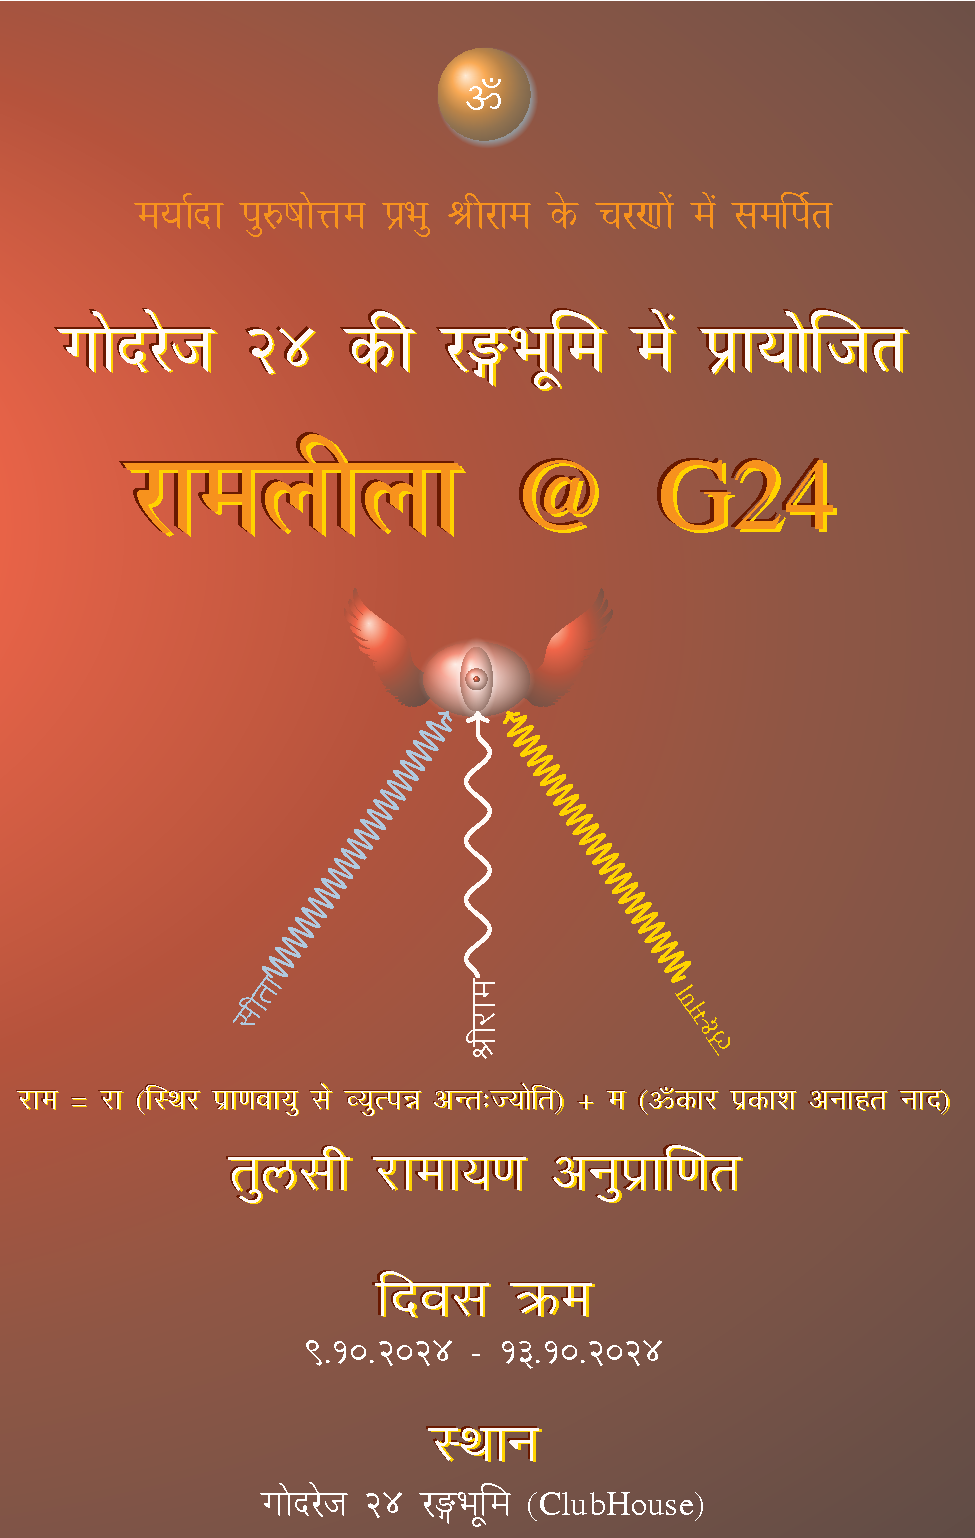
\includegraphics{front}
\end{center}

\renewcommand{\contentsname}{अनुक्रमणिका}
\renewcommand{\chaptername}{अध्याय}



\pagenumbering{gobble}
\tableofcontents*


\chapter[प्राक्कथन]{Preface}
\thispagestyle{empty}

\hspace{5mm} तन्त्र में ऊर्ध्वरित मन्त्रोच्चारण मात्र से किञ्चित मात्र भी हेतु की उपलब्धि नहीं हो पाती है। बाह्यडम्बर मात्र से यान्त्रिक गतिविधियों की मिथ्या पूर्ति की अभिसूचना मात्र होती है। अन्तःनिहित भाव से ही प्राण स्फुरण प्रक्रिया प्रारम्भ हो सकती है। उदाहरणतः बीज में वृक्षादि सूक्ष्म रूप से विद्यमान होते हैं। तत्नुसार तन्त्र विद्या के बीज मन्त्र में भी समस्त गुह्य क्रियाएँ सन्निहित हैं।  बीज के समयोचित एवं सुनियोजित अंकुरण व पोषण से कालान्तर में समस्त वृक्ष की उत्पत्ति होती है। उपयुक्त काल में फूल भी खिलते हैं एवं फलों से भी वृक्ष सुशोभित होता है। तदनुसार बीज मन्त्र के समुचित आवाहन से चैतन्य स्फुरण की प्रक्रिया स्वःघटित होती है एवं साधक का मेरुदण्ड स्वर्णिक आभा से आलोकित व सुशोभित होता है। कस्तूरी मृग की नाभि स्थित सदृश अविचल वायु की समस्त क्रियाएँ इन्हीं बीज मन्त्रों के प्रारूप में जीव में गुह्य संगठित हैं, जिनके अनवरत अभ्यास से साधकगण अघोर प्राणायामी पद को प्राप्त हो जाते हैं।   

\begin{center}
\small \bfseries नित्यानित्यवस्तुविचारादनित्यसंसारसुखदुःख विषयसमस्तक्षेत्र ममताबन्धक्षयो मोक्षः ॥
\end{center}

जब नित्य-अनित्य वस्तुओं के विषय में विचार करने से नश्वर संसार के सुख-दुःखात्मक समस्त विषयों से ममतारूपी बन्धन का विनाश हो जाये, तब ऐसी अवस्था को मोक्ष की संज्ञा दी गयी है। 

फलाकांक्षा से विमुक्त होकर क्रिया की परावस्था में पड़े रहना ही मोक्षावस्था है। 

क्रिया के समुचित व अनवरत अभ्यास से साधक गूढ़ प्राणायाम में पारंगत होकर अविचल स्थिर वायु की अद्भुत अवस्था को प्राप्त हो जाते हैं।  स्थिर वायु नाभि स्थल से प्रारम्भ होकर कूटस्थ त्रिनेत्र में समाहित हो जाती है, तदनुरूप साधक मन्त्र की गूढ़ावस्था चैतन्य स्वरुप में परिवर्तन प्रक्रिया का आत्मसाक्षी बन जाता है।  यही क्रिया की परावस्था अर्थात् मोक्षावस्था है।    

उदाहरणार्थ बीज मंत्र \textbf{क्रीं} के शब्द-विच्छेद द्वारा तीन अक्षर प्रकट होते हैं : \textbf{क} अर्थात् मस्तक का शीर्ष भाग सहस्रार, \textbf{र} अर्थात् अग्निबीज आज्ञा नेत्र एवं \textbf{इ} अर्थात् शक्ति स्वरुपा प्राण प्रकृति। 

तदनुसार बीज मंत्र \textbf{राम} में ॐकार स्पन्दन है। 

राम = रा (स्थिर प्राणवायु से व्युत्पन्न अन्तःज्योति) + म (ॐकार प्रकाश अनाहत नाद) 

\begin{center}
रम्यते अनेन इति रामः। \\
जो आनंद सिंधु सुखरासी। सीकर तें त्रैलोक सुपासी॥ \\
सो सुखधाम राम अस नामा। अखिल लोक दायक बिश्रामा॥ 
\end{center}

ॐकार की दिव्य ध्वनि चहुँ दिशा में गुंजायमान हो रही है तथा साधक परलौकिक आनंद से विभोर एवं सराबोर है। वो ॐकार से एकाकार हो जाता है।

'राम' पारलौकिक दिव्य अविचल प्राण वायु है। 

'लक्ष्मण' कूटस्थ लक्ष्य की ओर केंद्रित प्राण वायु है। 

कूटस्थित अवस्था यानि प्राण प्रतिष्ठा ही 'सीता' है।

जब इड़ा, पिंगला एवं सुषुम्ना नाड़ियों में प्राण वायु का प्रवाह थम जाता है तब साधक एक अनिर्वचनीय दिव्यानंदावस्था में स्थित हो जाता है। 

उसके अलौकिक दिव्य कम्पन से आच्छादित त्रिनेत्र में भगवान श्रीराम, लक्ष्मण एवं माँ सीता एकछत्र स्थापित हो जाते हैं।

अर्थात् प्राणायाम के सघन अभ्यास द्वारा चञ्चल प्राणवायु रूपी प्रकृति शक्ति ऊर्ध्वगामी होकर मस्तक अवस्थित कूटस्थ त्रिनेत्र में अविचल स्थिर हो जाती है। इस अवस्था में साधक को अनाहत चक्र के माध्यम से सतत् गुँजायमान ॐकार ध्वनि का दिव्य श्रवण एवं आज्ञा चक्र के माध्यम से बिन्दु के स्थिर स्वरुप का अलौकिक दिव्य दर्शन होता है।    



\chapter[बालकाण्ड]{BaalKand}
\thispagestyle{empty}


\hspace{5mm}अयोध्या नगरी में दशरथ नाम के राजा हुये जिनकी कौशल्या, कैकेयी और सुमित्रा नामक पत्नियाँ थीं। संतान प्राप्ति हेतु अयोध्यापति दशरथ ने अपने गुरु श्री वशिष्ठ की आज्ञा से पुत्रकामेष्टि यज्ञ करवाया जिसे कि ऋंगी ऋषि ने सम्पन्न किया। भक्तिपूर्ण आहुतियाँ पाकर अग्निदेव प्रसन्न हुये और उन्होंने स्वयं प्रकट होकर राजा दशरथ को हविष्यपात्र (खीर, पायस) दिया जिसे कि उन्होंने अपनी तीनों पत्नियों में बाँट दिया। खीर के सेवन के परिणामस्वरूप कौशल्या के गर्भ से राम का, कैकेयी के गर्भ से भरत का तथा सुमित्रा के गर्भ से लक्ष्मण और शत्रुघ्न का जन्म हुआ।

राजकुमारों के बड़े होने पर आश्रम की राक्षसों से रक्षा हेतु ऋषि विश्वामित्र राजा दशरथ से राम और लक्ष्मण को मांग कर अपने साथ ले गये। 


\begin{center}
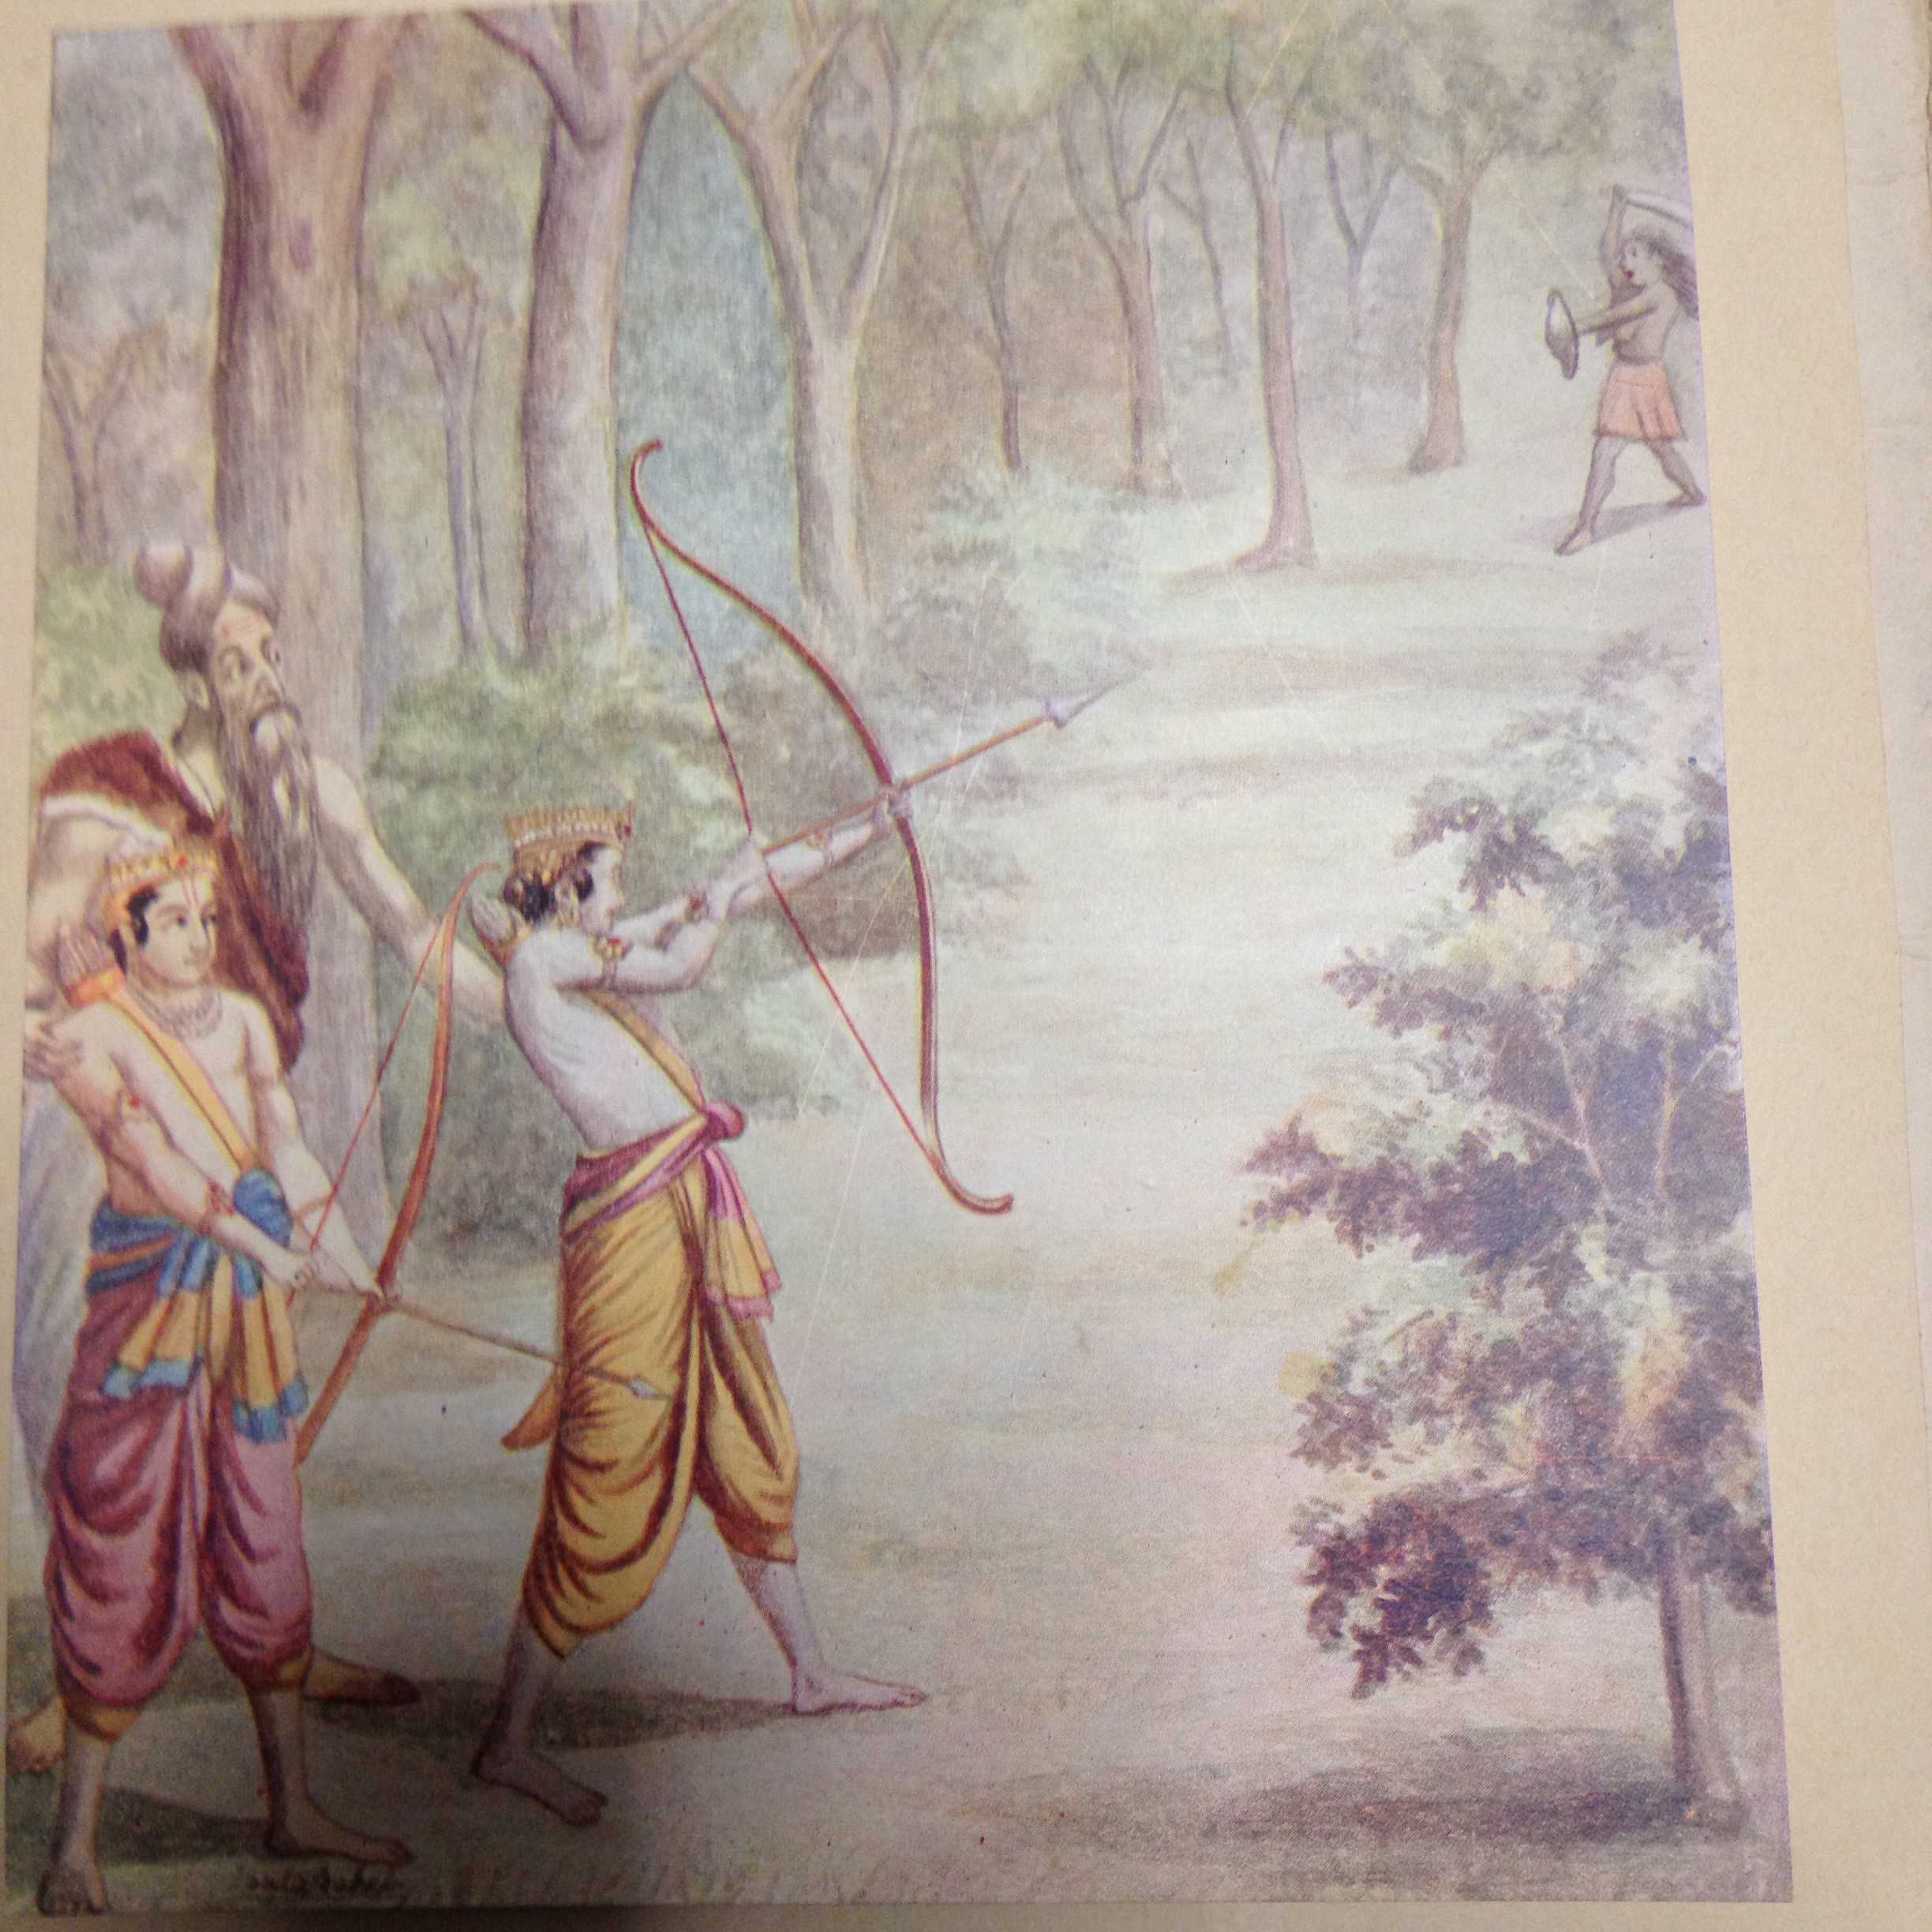
\includegraphics[scale=0.05]{Rama_Killing_Demon_Tataka.jpeg}
\end{center}

राम ने ताड़का और सुबाहु जैसे राक्षसों को मार डाला और मारीच को बिना फर वाले बाण से मार कर समुद्र के पार भेज दिया। 




उधर लक्ष्मण ने राक्षसों की सारी सेना का संहार कर डाला। धनुषयज्ञ हेतु राजा जनक के निमंत्रण मिलने पर विश्वामित्र राम और लक्ष्मण के साथ उनकी नगरी मिथिला (जनकपुर) आ गये।


 रास्ते में राम ने गौतम मुनि की स्त्री अहल्या का उद्धार किया। मिथिला में राजा जनक की पुत्री सीता जिन्हें कि जानकी के नाम से भी जाना जाता है का स्वयंवर का भी आयोजन था जहाँ कि जनकप्रतिज्ञा के अनुसार शिवधनुष को तोड़ कर राम ने सीता से किया। राम और सीता के विवाह के साथ ही साथ गुरु वशिष्ठ और गुरु विश्वामित्र के परामर्श से भरत का माण्डवी से, लक्ष्मण का उर्मिला से और शत्रुघ्न का श्रुतकीर्ति से विवाह संपन्न किया गया। 
 
 \begin{center}
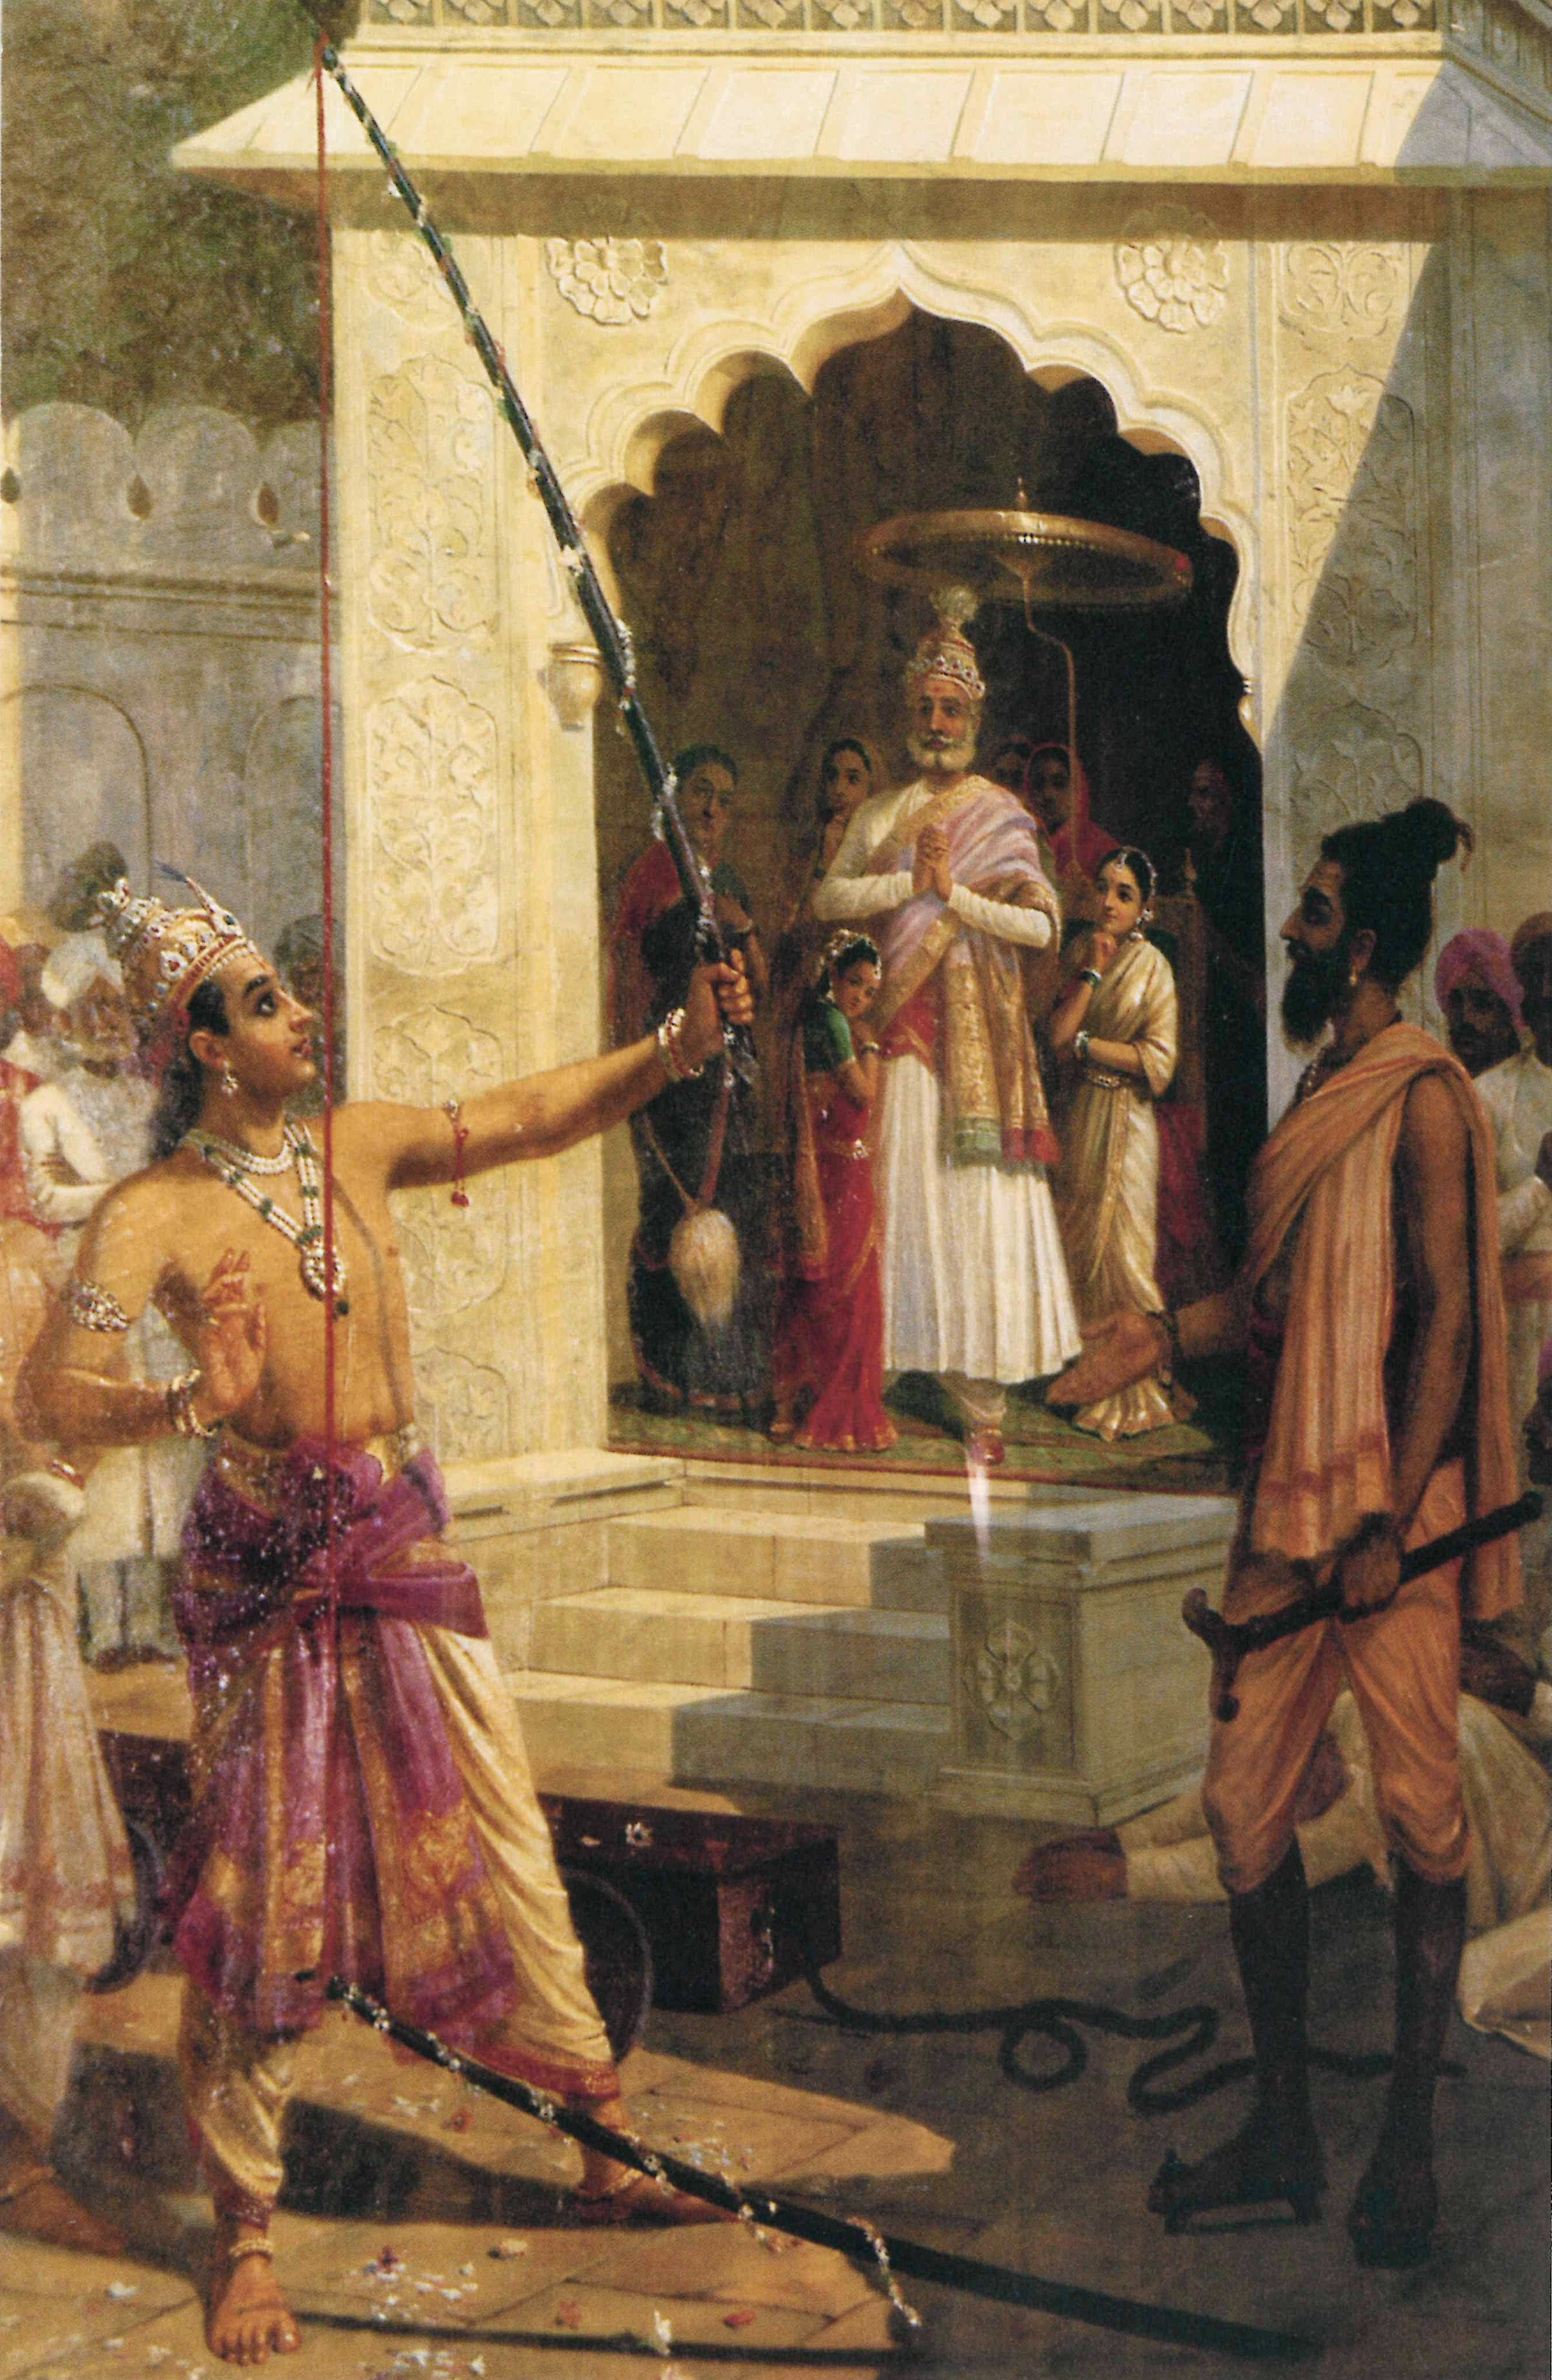
\includegraphics[scale=0.05]{Ravi_Varma-Rama-breaking-bow.jpg}
\end{center}



\chapter[अयोध्याकाण्ड]{AyodhyaKand}
\thispagestyle{empty}


\hspace{5mm}राम के विवाह के कुछ समय पश्चात् राजा दशरथ ने राम का राज्याभिषेक करना चाहा। इस पर देवता लोगों को चिंता हुई कि राम को राज्य मिल जाने पर रावण का वध असम्भव हो जायेगा। व्याकुल होकर उन्होंने देवी सरस्वती से किसी प्रकार के उपाय करने की प्रार्थना की। सरस्वती ने मन्थरा, जो कि कैकेयी की दासी थी, की बुद्धि को फेर दिया। मन्थरा की सलाह से कैकेयी कोपभवन में चली गई। 

 \begin{center}
\includegraphics[scale=0.03]{Kaikeyi_vilap.jpg}
\end{center}

दशरथ जब मनाने आये तो कैकेयी ने उनसे वरदान मांगे कि भरत को राजा बनाया जाये और राम को चौदह वर्षों के लिये वनवास में भेज दिया जाये।

राम के साथ सीता और लक्ष्मण भी वन चले गये। ऋंगवेरपुर में निषादराज गुह ने तीनों की बहुत सेवा की। कुछ आनाकानी करने के बाद केवट ने तीनों को गंगा नदी के पार उतारा| प्रयाग पहुँच कर राम ने भरद्वाज मुनि से भेंट की। वहाँ से राम यमुना स्नान करते हुए वाल्मीकि ऋषि के आश्रम पहुँचे। वाल्मीकि से हुई मन्त्रणा के अनुसार राम, सीता और लक्ष्मण चित्रकूट में निवास करने लगे।

 \begin{center}
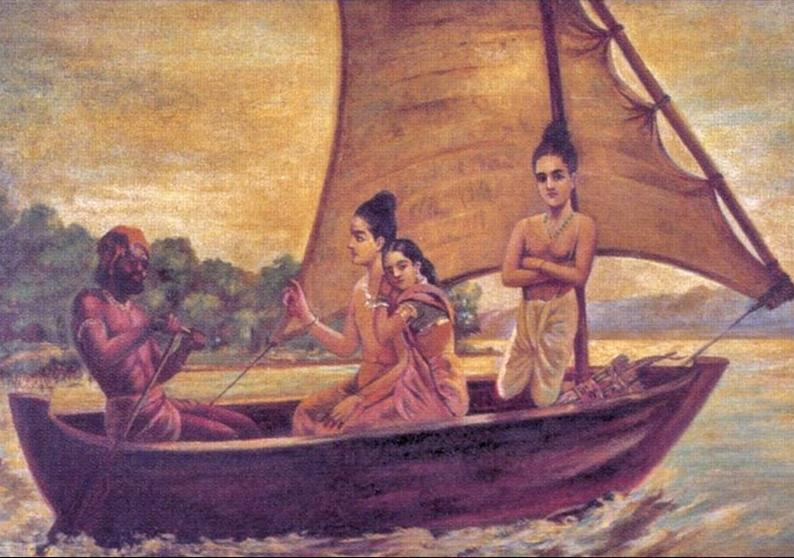
\includegraphics[scale=0.4]{Sree_Rama_Crossing_Sarayu_river.jpg}
\end{center}


अयोध्या में पुत्र के वियोग के कारण दशरथ का स्वर्गवास हो गया। वशिष्ठ ने भरत और शत्रुघ्न को उनके ननिहाल से बुलवा लिया। वापस आने पर भरत ने अपनी माता कैकेयी की, उसकी कुटिलता के लिये, बहुत भर्तस्ना की और गुरुजनों के आज्ञानुसार दशरथ की अन्त्येष्टि क्रिया कर दिया। भरत ने अयोध्या के राज्य को अस्वीकार कर दिया और राम को मना कर वापस लाने के लिये समस्त स्नेहीजनों के साथ चित्रकूट चले गये। कैकेयी को भी अपने किये पर अत्यंत पश्चाताप हुआ। सीता के माता-पिता सुनयना एवं जनक भी चित्रकूट पहुँचे। भरत तथा अन्य सभी लोगों ने राम के वापस अयोध्या जाकर राज्य करने का प्रस्ताव रखा जिसे कि राम ने, पिता की आज्ञा पालन करने और रघुवंश की रीति निभाने के लिये, अमान्य कर दिया।

भरत अपने स्नेही जनों के साथ राम की पादुका को साथ लेकर वापस अयोध्या आ गये। उन्होंने राम की पादुका को राज सिंहासन पर विराजित कर दिया स्वयं नन्दिग्राम में निवास करने लगे। 



\chapter[अरण्यकाण्ड]{AranyaKand}
\thispagestyle{empty}



\hspace{5mm}कुछ काल के पश्चात राम ने चित्रकूट से प्रयाण किया तथा वे अत्रि ऋषि के आश्रम पहुंचे। अत्रि ने राम की स्तुति की और उनकी पत्नी अनसूया ने सीता को पातिव्रत धर्म के मर्म समझाये। 

 \begin{center}
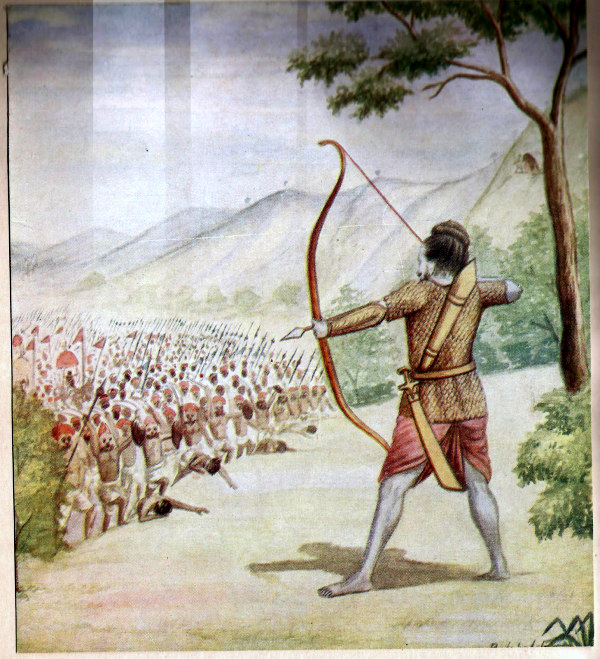
\includegraphics[scale=0.27]{Rama_Fights_the_Demons.jpg}
\end{center}

वहां से फिर राम ने आगे प्रस्थान किया और शरभंग मुनि से भेंट की। शरभंग मुनि केवल राम के दर्शन की कामना से वहां निवास कर रहे थे अतः राम के दर्शनों की अपनी अभिलाषा पूर्ण हो जाने से योगाग्नि से अपने शरीर को जला डाला और ब्रह्मलोक को गमन किया। और आगे बढ़ने पर राम को स्थान स्थान पर हड्डियों के ढेर दिखाई पड़े जिनके विषय में मुनियों ने राम को बताया कि राक्षसों ने अनेक मुनियों को खा डाला है और उन्हीं मुनियों की हड्डियां हैं। इस पर राम ने प्रतिज्ञा की कि वे समस्त राक्षसों का वध करके पृथ्वी को राक्षस विहीन कर देंगे। राम और आगे बढ़े और पथ में सुतीक्ष्ण, अगस्त्य आदि ऋषियों से भेंट करते हुए दण्डक वन में प्रवेश किया जहां पर उनकी भेंट जटायु से हुई। राम ने पंचवटी को अपना निवास स्थान बनाया।

 \begin{center}
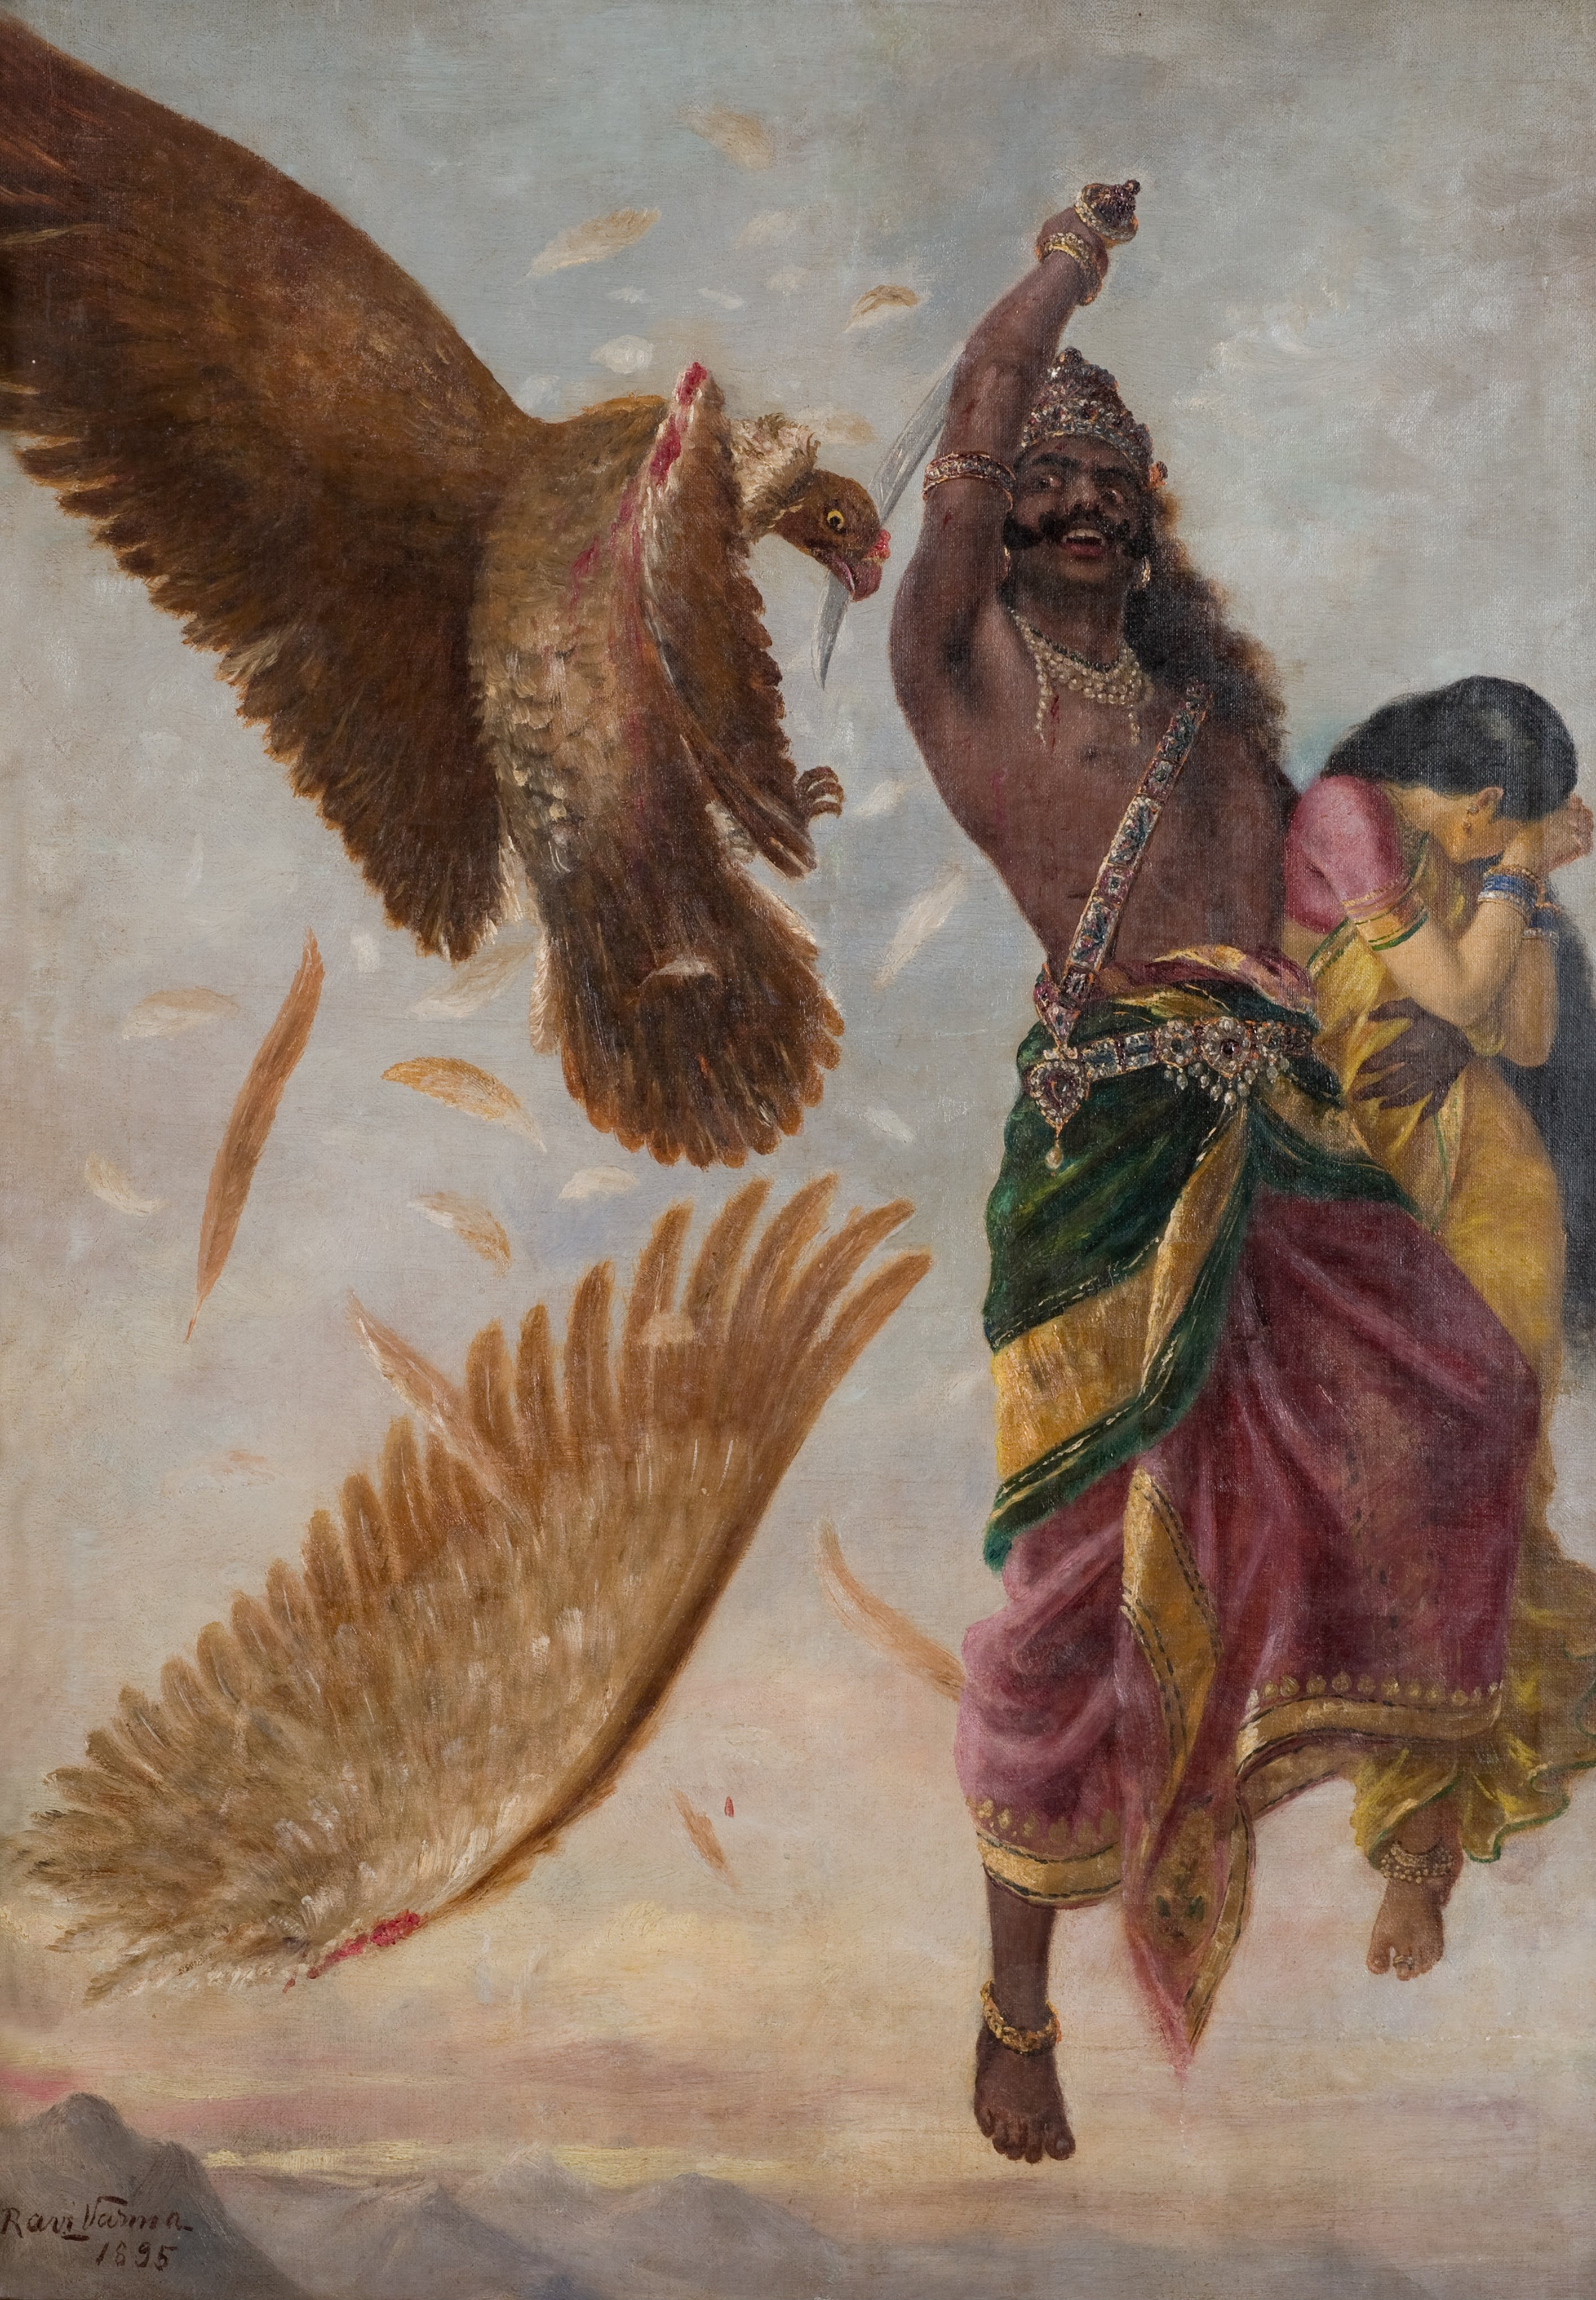
\includegraphics[scale=0.05]{Ravi_Varma-Ravana_Sita_Jathayu.jpg}
\end{center}

पंचवटी में रावण की बहन शूर्पणखा ने आकर राम से प्रणय निवेदन-किया। राम ने यह कह कर कि वे अपनी पत्नी के साथ हैं और उनका छोटा भाई अकेला है उसे लक्ष्मण के पास भेज दिया। लक्ष्मण ने उसके प्रणय-निवेदन को अस्वीकार करते हुए शत्रु की बहन जान कर उसके नाक और कान काट लिये। शूर्पणखा ने खर-दूषण से सहायता की मांग की और वह अपनी सेना के साथ लड़ने के लिये आ गया। लड़ाई में राम ने खर-दूषण और उसकी सेना का संहार कर डाला। शूर्पणखा ने जाकर अपने भाई रावण से शिकायत की। रावण ने बदला लेने के लिये मारीच को स्वर्णमृग बना कर भेजा जिसकी छाल की मांग सीता ने राम से की। लक्ष्मण को सीता के रक्षा की आज्ञा दे कर राम स्वर्णमृग रूपी मारीच को मारने के लिये उसके पीछे चले गये। मारीच राम के हाथों मारा गया पर मरते मरते मारीच ने राम की आवाज बना कर 'हे लक्ष्मण' का क्रन्दन किया जिसे सुन कर सीता ने आशंकावश होकर लक्ष्मण को राम के पास भेज दिया। लक्ष्मण के जाने के बाद अकेली सीता का रावण ने छलपूर्वक हरण कर लिया और अपने साथ लंका ले गया। रास्ते में जटायु ने सीता को बचाने के लिये रावण से युद्ध किया और रावण ने उसके पंख काटकर उसे अधमरा कर दिया।



सीता को न पा कर राम अत्यंत दुखी हुए और विलाप करने लगे। रास्ते में जटायु से भेंट होने पर उसने राम को रावण के द्वारा अपनी दुर्दशा होने व सीता को हर कर दक्षिण दिशा की ओर ले जाने की बात बताई। ये सब बताने के बाद जटायु ने अपने प्राण त्याग दिये और राम उसका अंतिम संस्कार करके सीता की खोज में सघन वन के भीतर आगे बढ़े। रास्ते में राम ने दुर्वासा के शाप के कारण राक्षस बने गन्धर्व कबन्ध का वध करके उसका उद्धार किया और शबरी के आश्रम जा पहुंचे जहां पर कि उसके द्वारा दिये गये जूठे बेरों को उसके भक्ति के वश में होकर खाया| इस प्रकार राम सीता की खोज में सघन वन के अंदर आगे बढ़ते गये। 


\chapter[किष्किन्धाकाण्ड]{KishkindhaKand}
\thispagestyle{empty}



\hspace{5mm}श्री राम ऋष्यमूक पर्वत के निकट आ गये। उस पर्वत पर अपने मंत्रियों सहित सुग्रीव रहता था। सुग्रीव ने, इस आशंका में कि कहीं बालि ने उसे मारने के लिये उन दोनों वीरों को न भेजा हो, हनुमान को श्री राम और लक्ष्मण के विषय में जानकारी लेने के लिये ब्राह्मण के रूप में भेजा। यह जानने के बाद कि उन्हें बालि ने नहीं भेजा है हनुमान ने श्री राम और सुग्रीव में मित्रता करवा दी। 

 \begin{center}
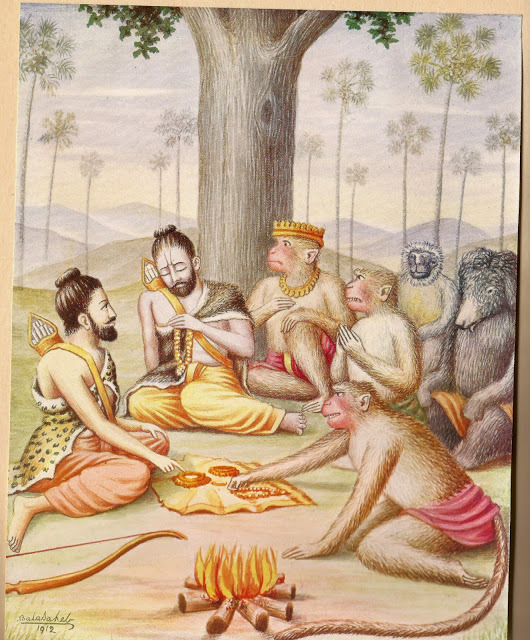
\includegraphics[scale=0.27]{Rama_Meets_Sugreeva.jpg}
\end{center}

सुग्रीव ने श्री राम को सान्त्वना दी कि जानकी जी मिल जायेंगीं और उन्हें खोजने में वह सहायता देगे। साथ ही अपने भाई बालि के अपने ऊपर किये गये अत्याचार के विषय में बताया। श्री राम ने बालि का वध कर के सुग्रीव को किष्किन्धा का राज्य तथा बालि के पुत्र अंगद को युवराज का पद दे दिया।



राज्य प्राप्ति के बाद सुग्रीव विलास में लिप्त हो गये और वर्षा तथा शरद् ऋतु बीत गए । राम के नाराजगी पर सुग्रीव ने वानरों को सीता की खोज के लिये भेजा। सीता की खोज में गये वानरों को एक गुफा में एक तपस्विनी के दर्शन हुए। तपस्विनी ने खोज दल को योगशक्ति से समुद्रतट पर पहुँचा दिया जहाँ पर उनकी भेंट सम्पाती से हुई। सम्पाती ने वानरों को बताया कि रावण ने सीता को लंका की अशोकवाटिका में रखा है। जाम्बवन्त ने हनुमान को समुद्र लांघने के लिये कहा किन्तु हनुमान जी इतनी दूर कैसे जाएंगे । तब हनुमान जी ने जाम्बवन्त जी से पुछा कि " मैं इतनी दूर कैसे जा पाऊंगा।" तब जाम्बवन्त जी ने उनकी शक्तियों को याद दिलाया और बताया कि उन्हें श्री भृगुवंशी जी को परेशान करते थे जिससे तंग आकर उन्होंने हनुमान को शाप दे दिया की,"आप अपने बल और तेज को सदा के लिए भूल जाएं लेकिन जब कोई आपको आपकी शक्तियां याद कराएगा तभी आप उसका उपयोग कर सकोगे।" फिर वे आगे बढ़कर उन्होंने अपनी शक्तियों का अहसास किया। 

 \begin{center}
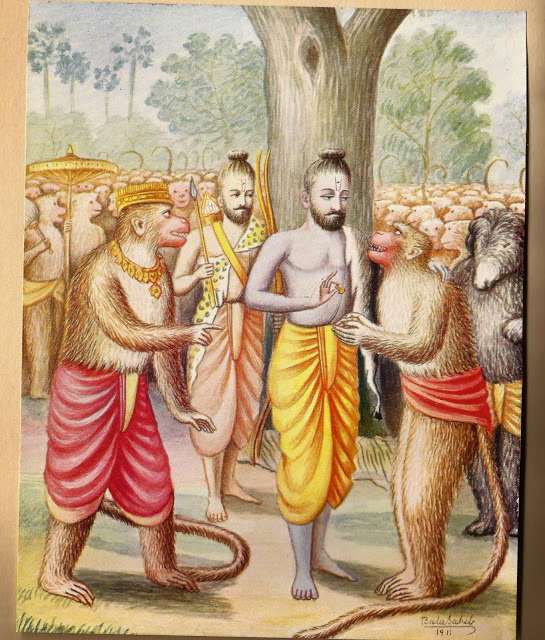
\includegraphics[scale=0.27]{The_Signet_Ring.jpg}
\end{center}


\chapter[सुन्दरकाण्ड]{SundarKand}
\thispagestyle{empty}


\hspace{5mm}हनुमान जी ने लंका की ओर प्रस्थान किया। सुरसा ने हनुमान जी की परीक्षा ली और उसे योग्य तथा सामर्थ्यवान पाकर आशीर्वाद दिया। मार्ग में हनुमान जी ने छाया पकड़ने वाली राक्षसी का वध किया और लंकिनी पर प्रहार करके लंका में प्रवेश किया। उनकी विभीषण से भेंट हुई। जब हनुमान जी अशोकवाटिका में पहुँचे तो रावण सीता को धमका रहा था। रावण के जाने पर त्रिजटा ने सीता को सान्त्वना दी। एकान्त होने पर हनुमान जी ने सीता से भेंट करके उन्हें राम की मुद्रिका दी। 

 \begin{center}
\includegraphics[scale=0.05]{Hanuman_Encounters_Sita_in_Ashokavana.jpg}
\end{center}

हनुमान जी ने अशोकवाटिका का विध्वंस करके रावण के पुत्र अक्षय कुमार का वध कर दिया। मेघनाथ हनुमान को नागपाश में बांध कर रावण की सभा में ले गया। रावण के प्रश्न के उत्तर में हनुमान ने अपना परिचय राम के दूत के रूप में दिया। रावण ने हनुमान जी की पूँछ में तेल में डूबा हुआ कपड़ा बांध कर आग लगा दिया इस पर हनुमान जी ने लंका का दहन कर दिया।

 \begin{center}
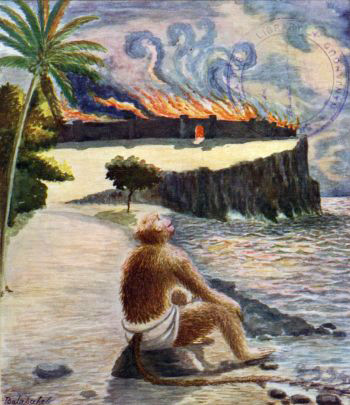
\includegraphics[scale=2]{Hanuman_Watches_Lanka_Burn.jpg}
\end{center}

हनुमान जी सीता के पास पहुँचे। सीता ने अपनी चूड़ामणि दे कर उन्हें विदा किया। वे वापस समुद्र पार आकर सभी वानरों से मिले और सभी वापस सुग्रीव के पास चले गये। हनुमान के कार्य से राम अत्यंत प्रसन्न हुए। राम वानरों की सेना के साथ समुद्रतट पर पहुँचे। उधर विभीषण ने रावण को समझाया कि राम से बैर न लें इस पर रावण ने विभीषण को अपमानित कर लंका से निकाल दिया। विभीषण राम के शरण में आ गया और राम ने उसे लंका का राजा घोषित कर दिया। राम ने समुद्र से रास्ता देने की विनती की। विनती न मानने पर राम ने क्रोध किया और उनके क्रोध से भयभीत होकर समुद्र ने स्वयं आकर राम की विनती करने के पश्चात् नल और नील के द्वारा पुल बनाने का उपाय बताया। 

\chapter[लङ्काकाण्ड]{LankaKand}
\thispagestyle{empty}

\hspace{5mm}जाम्बवन्त के आदेश से नल-नील दोनों भाइयों ने वानर सेना की सहायता से समुद्र पर पुल बांध दिया। श्री राम ने श्री रामेश्वर की स्थापना करके भगवान शंकर की पूजा की और सेना सहित समुद्र के पार उतर गये।

 \begin{center}
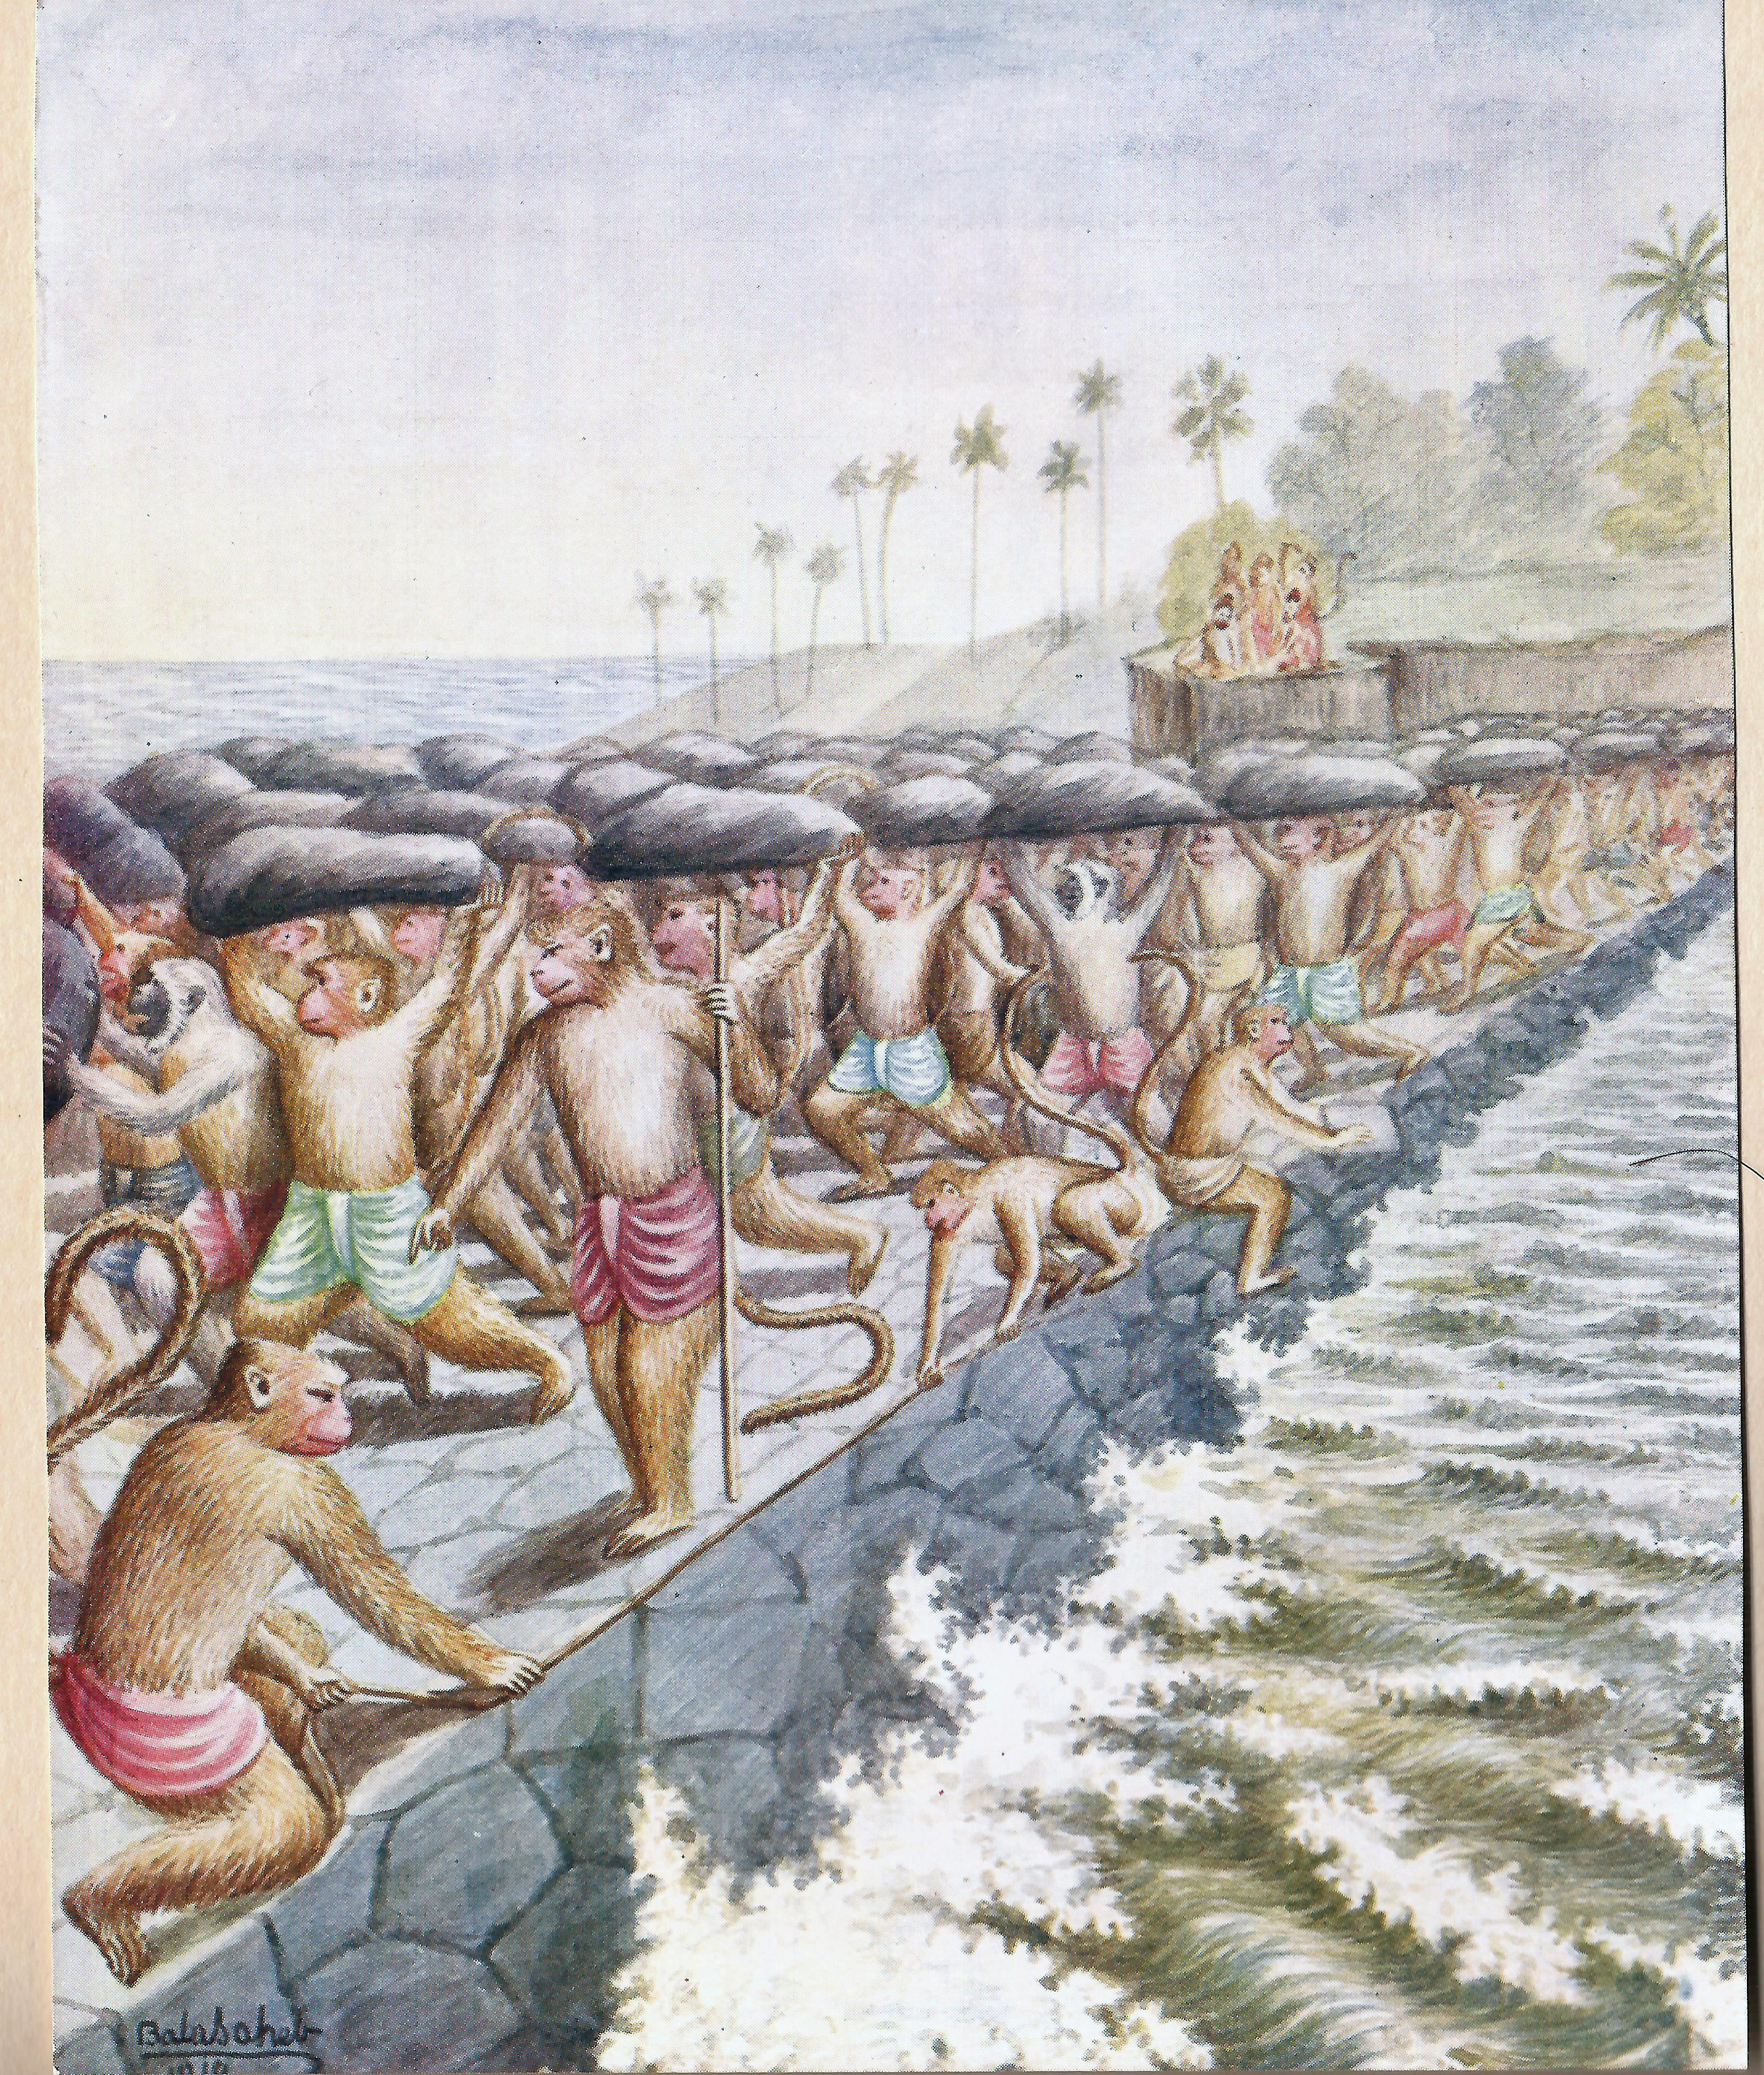
\includegraphics[scale=0.05]{Building_a_Bridge_to_Sri_Lanka.jpg}
\end{center}

समुद्र के पार जाकर राम ने डेरा डाला। पुल बंध जाने और राम के समुद्र के पार उतर जाने के समाचार से रावण मन में अत्यंत व्याकुल हुआ। मन्दोदरी के राम से बैर न लेने के लिये समझाने पर भी रावण का अहंकार नहीं गया। इधर राम अपनी वानरसेना के साथ सुबेल पर्वत पर निवास करने लगे। अंगद राम के दूत बन कर लंका में रावण के पास गये और उसे राम के शरण में आने का संदेश दिया किन्तु रावण ने नहीं माना।



शांति के सारे प्रयास असफल हो जाने पर युद्ध आरम्भ हो गया। लक्ष्मण और मेघनाद के मध्य घोर युद्ध हुआ। शक्तिबाण के वार से लक्ष्मण मूर्छित हो गये। उनके उपचार के लिये हनुमान सुषेण वैद्य को ले आये और संजीवनी लाने के लिये चले गये। गुप्तचर से समाचार मिलने पर रावण ने हनुमान के कार्य में बाधा के लिये कालनेमि को भेजा जिसका हनुमान ने वध कर दिया। औषधि की पहचान न होने के कारण हनुमान पूरे पर्वत को ही उठा कर वापस चले। मार्ग में हनुमान को राक्षस होने के सन्देह में भरत ने बाण मार कर मूर्छित कर दिया परन्तु यथार्थ जानने पर अपने बाण पर बिठा कर वापस लंका भेज दिया। इधर औषधि आने में विलम्ब देख कर राम प्रलाप करने लगे। सही समय पर हनुमान औषधि लेकर आ गये और सुषेण के उपचार से लक्ष्मण स्वस्थ हो गये।


 \begin{center}
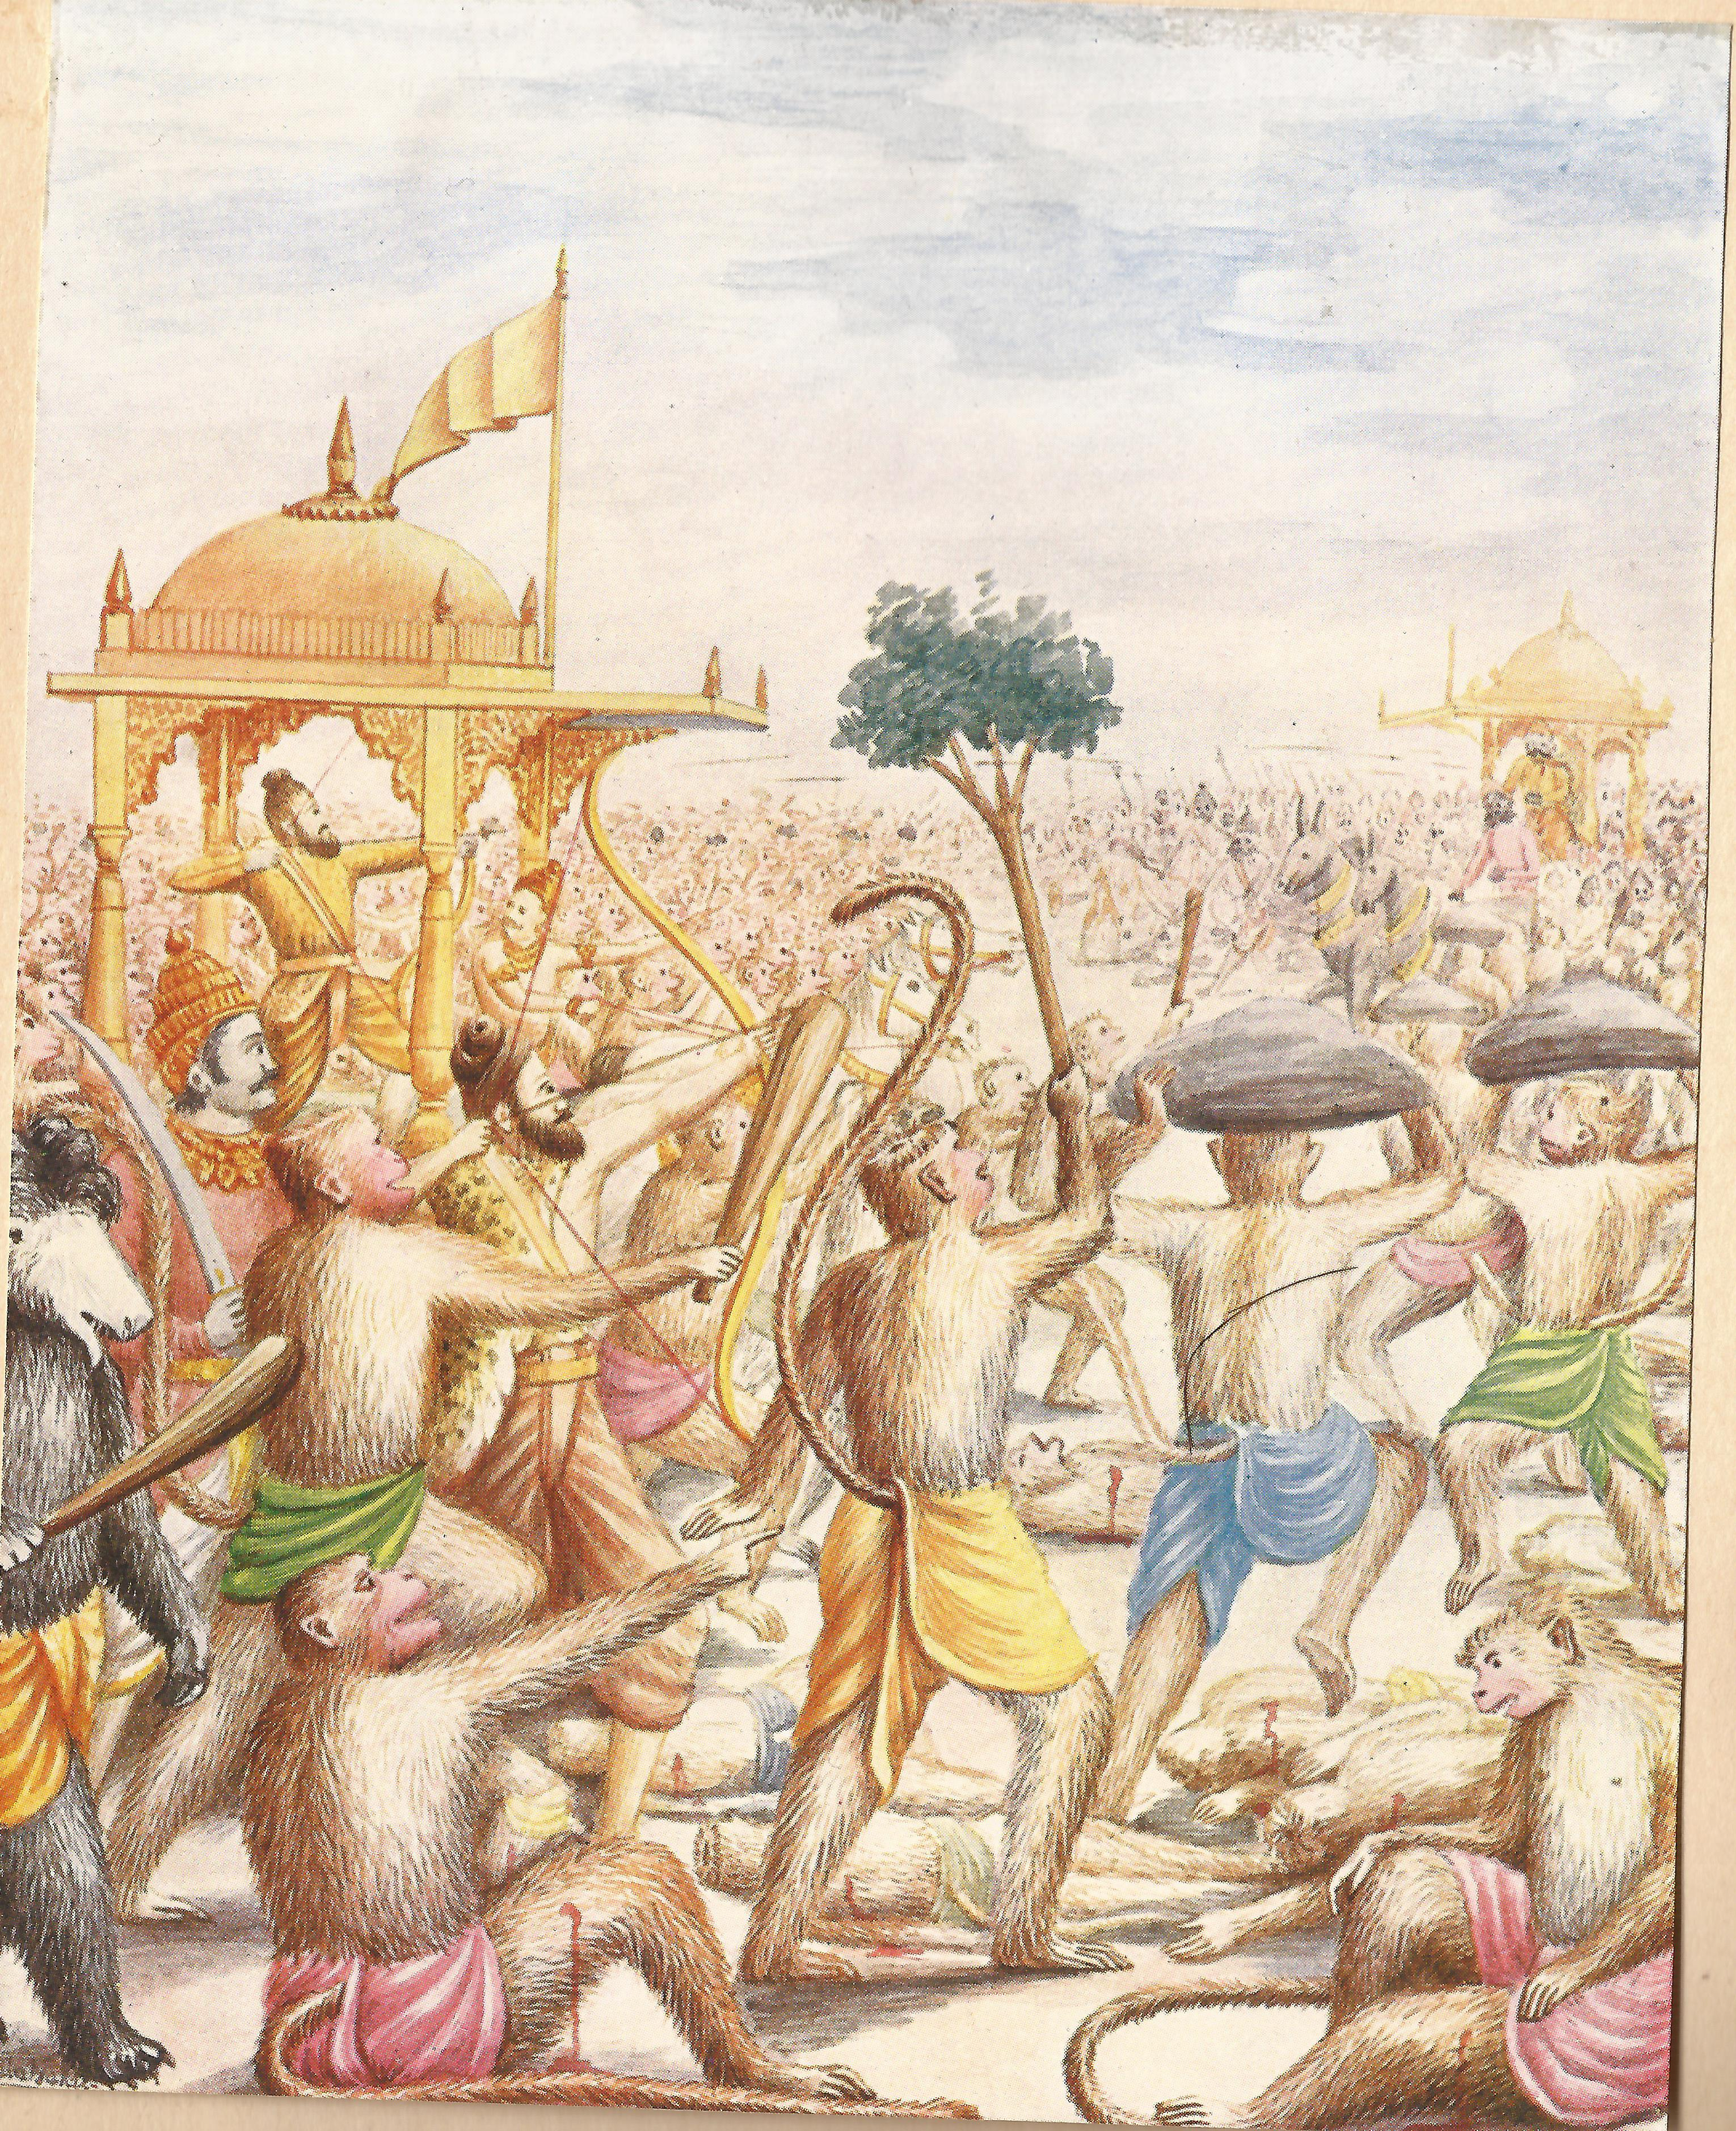
\includegraphics[scale=0.5]{ravan-vadh.jpg}
\end{center}

रावण ने युद्ध के लिये कुम्भकर्ण को जगाया। कुम्भकर्ण ने भी राम के शरण में जाने की असफल मन्त्रणा दी। युद्ध में कुम्भकर्ण ने राम के हाथों परमगति प्राप्त की। लक्ष्मण ने मेघनाद से युद्ध करके उसका वध कर दिया। राम और रावण के मध्य अनेकों घोर युद्ध हुए और अन्त में रावण राम के हाथों मारा गया। विभीषण को लंका का राज्य सौंप कर राम सीता और लक्ष्मण के साथ पुष्पकविमान पर चढ़ कर अयोध्या के लिये प्रस्थान किया। 



\chapter[उत्तरकाण्ड]{UttarKand}
\thispagestyle{empty}

\hspace{5mm}सीता, लक्ष्मण और समस्त वानर सेना के साथ राम अयोध्या वापस पहुँचे। राम का भव्य स्वागत हुआ, भरत के साथ सर्वजनों में आनन्द व्याप्त हो गया। वेदों और शिव की स्तुति के साथ राम का राज्याभिषेक हुआ। वानरों की विदाई दी गई। राम ने प्रजा को उपदेश दिया और प्रजा ने कृतज्ञता प्रकट की। फिर प्रजा ने सीता के चरित्र पर आरोप लगाया और राम द्वारा प्रजा के लिए सीता का त्याग किया गया । त्याग के बाद सीता वन चली गईं और महाऋषि वाल्मीकि के आश्रम में रहने लगीं । उस वक़्त वो गर्भ से थीं । समय आने पर चारों भाइयों के दो दो पुत्र हुए। लव कुश के बड़े होने पर वो अपनी माता के लिए न्याय मागने अयोध्या आये परंतु प्रजा की इच्छा के कारण सीता को फिर परीक्षा के लिए बुलाया गया और वे अपनी परीक्षा देकर धरती माता के साथ धरती में समा गयीं । काल के वचन के कारण राम ने लक्ष्मण का त्याग किया और पुत्रों के बड़े होने पर उन सब में राज्य का बंटवारा कर अपने धाम को चल दिये रामराज्य एक आदर्श बन गया। 




\vspace{1mm}

\hspace{5mm} कालांतर में साधक को ये सत्य विदित होता है कि यह एक सार्वभौम क्रिया है एवं इसका प्रत्येक 'शब्द' अक्षुण्ण, पारलौकिक एवं अक्षय है जिसका प्रादुर्भाव सामान्यतः अगोचर है। ये सर्वदा गुंजायमान है एवं सिद्धों द्वारा इनके अनवरत तथा अद्भुत कालातीत जप का श्रवण साधक को उपयुक्त काल में होता है। 


\end{document}
